% =============================================================================
% 5. EXPERIMENTAL RESULTS AND PRACTICAL ENGINEERING ANALYSIS
% =============================================================================
\section{Experimental Results and Practical Engineering Analysis}
\label{sec:results}

This section evaluates BioDINO-Edge against operational edge deployment requirements. We first benchmark classification accuracy against few-shot baselines on controlled and in-the-wild datasets (Section~\ref{sec:comparative_results}) and verify statistical significance (Section~\ref{sec:significance}). We then evaluate the contribution of each framework component (Section~\ref{sec:ablation}), measure on-device latency and memory footprints across embedded target hardware (Section~\ref{sec:edge_hardware}), test robustness against sensor noise and parameter variations (Section~\ref{sec:calibration}), and examine per-class diagnostic failure patterns (Section~\ref{sec:per_class}).

% -----------------------------------------------------------------------------
% 5.1 Primary Benchmark Performance and Baseline Evaluation
% -----------------------------------------------------------------------------
\subsection{Primary Benchmark Performance and Baseline Evaluation}
\label{sec:comparative_results}

To benchmark diagnostic accuracy under controlled conditions, Table~\ref{tab:comparative} compares BioDINO-Edge against representative zero-shot and few-shot baseline paradigms. All methods are evaluated across identical support/query partitions, random seeds, and shot counts ($K \in \{1, 5\}$). Extended $K$-shot curves appear in \ref{app:shot_ladder} (Table~\ref{tab:shot_ladder}).

\begin{table*}[htbp]
\caption{Controlled comparison with few-shot baseline paradigms on PlantVillage under identical frozen representations, splits, and seeds (single-view reference features).}
\label{tab:comparative}
\centering

\footnotesize
\setlength{\tabcolsep}{3.5pt}
\begin{tabularx}{\textwidth}{@{}>{\raggedright\arraybackslash}X *{4}{>{\centering\arraybackslash}p{2.6cm}}@{}}
\toprule
& \multicolumn{2}{c}{\textbf{5-way accuracy (\%) ($\uparrow$)}} & \multicolumn{2}{c}{\textbf{11-class, 5-shot (\%) ($\uparrow$)}} \\
\cmidrule(lr){2-3}\cmidrule(lr){4-5}
\textbf{Method} & \textbf{1-shot} & \textbf{5-shot} & \textbf{Accuracy} & \textbf{Macro F1} \\
\midrule
Zero-shot BioCLIP~\cite{stevens2024bioclip} & 38.89$\pm$12.78 & 38.86$\pm$12.79 & 19.18$\pm$0.02 & 18.49 \\
Tip-Adapter~\cite{zhang2022tip} & 45.15$\pm$13.42 & 68.63$\pm$12.80 & 49.97$\pm$1.62 & 46.54 \\
Prototypical Networks~\cite{snell2017prototypical} & 88.44$\pm$9.13 & 97.45$\pm$2.03 & 93.28$\pm$1.24 & 92.47 \\
BioDINO-Edge (inductive, ours) & \underline{88.45$\pm$9.12} & \underline{97.96$\pm$1.85} & \underline{95.08$\pm$1.27} & \underline{94.51} \\
BioDINO-Edge (transductive, ours) & \textbf{93.42$\pm$6.83} & \textbf{98.77$\pm$1.68} & \textbf{97.41$\pm$0.71} & \textbf{97.09} \\
\bottomrule
\end{tabularx}

\vspace{3pt}
\begin{minipage}{\textwidth}
\footnotesize
\textit{Notes.} Bold denotes the best performance in each column; underline denotes second-best. $(\uparrow)$ indicates metrics where higher values are better.
\end{minipage}
\end{table*}

\textbf{Engineering interpretation of baseline performance.} As shown in Table~\ref{tab:comparative}, BioDINO-Edge improves diagnostic accuracy across all few-shot regimes. In the inductive setting, regularized Fisher-LDA projection suppresses common vegetative variance, reaching 95.08\% accuracy. Incorporating transductive anchor recalibration further raises accuracy to 97.41\%, executing entirely on edge CPUs without backpropagation. In contrast, standard unregularized distance metrics underperform because treating all 896 embedding dimensions uniformly leaves predictions vulnerable to dominant leaf veins and glare, while general text prompts in zero-shot adapters lack spatial lesion specificity.

To isolate the impact of our adaptation framework from feature dimensionality and transductive access, Table~\ref{tab:fair_baselines} compares all baselines on identical 896-D features and identical episodes. Following linear-probe evaluations on frozen embeddings~\cite{tian2020rethinking}, we include regularized multinomial logistic regression; we add a closed-form ridge-regression probe in the spirit of differentiable closed-form few-shot solvers~\cite{bertinetto2019r2d2}. Across all inductive comparators on the 896-D features, BioDINO-Edge consistently outperforms Ridge regression, logistic regression, Tip-Adapter, and Prototypical Networks.

Because BioDINO-Edge incorporates transductive recalibration, we also evaluate standard transductive baselines under full-batch query access. In this offline setting with the entire test set visible simultaneously, our re-implementation of LaplacianShot~\cite{ziko2020laplacian} reaches 98.49\% on 11-class PlantVillage (1.08\,pp above BioDINO-Edge), whereas our re-implementations of TIM~\cite{boudiaf2020transductive} and prototype rectification~\cite{liu2020bdcspn} achieve lower accuracy. We also tested whether our regularized Fisher projection could serve as a preprocessing front-end for LaplacianShot. Running Laplacian propagation in the Fisher-projected subspace drops accuracy by 5.7\,pp (from 98.49\% down to 92.84\%). This drop occurs because Fisher-LDA projects the 896 dimensions onto $C-1$ discriminant axes to maximize global class separation, which removes the fine-grained local neighborhood manifold that graph Laplacian smoothing relies on.

\begin{table*}[htbp]
\caption{Comparison with inductive and transductive few-shot baselines on identical 896-D single-view features and episodes (PlantVillage).}
\label{tab:fair_baselines}
\centering

\footnotesize
\setlength{\tabcolsep}{4pt}
\begin{tabularx}{\textwidth}{@{}>{\raggedright\arraybackslash}X *{4}{>{\centering\arraybackslash}p{2.3cm}}@{}}
\toprule
\textbf{Method (features)} & \textbf{5-way 1-shot} & \textbf{5-way 5-shot} & \textbf{11-class, 5-shot} & \textbf{11-class F1} \\
\midrule
\multicolumn{5}{@{}l}{\textit{Inductive: training-free and closed-form linear probes}}\\
Tip-Adapter (512-D BioCLIP, as published) & 45.15$\pm$13.42 & 68.63$\pm$12.80 & 49.97$\pm$1.62 & 46.54 \\
Tip-Adapter (896-D, ours) & -- & 73.02$\pm$12.21 & 55.60$\pm$1.67 & 51.15 \\
Ridge classifier (896-D) & -- & 97.74$\pm$1.82 & 93.83$\pm$1.08 & 92.47 \\
Multinomial logistic (896-D) & -- & 97.67$\pm$1.82 & 93.63$\pm$1.02 & 92.52 \\
Prototypical Networks (896-D) & 88.44$\pm$9.13 & 97.45$\pm$2.03 & 93.28$\pm$1.24 & 92.47 \\
BioDINO-Edge inductive (896-D) & \underline{88.45$\pm$9.12} & 97.96$\pm$1.85 & 95.08$\pm$1.27 & 94.51 \\
\midrule
\multicolumn{5}{@{}l}{\textit{Transductive: same features, same episodes}}\\
Prototype rectification~\cite{liu2020bdcspn} (896-D) & -- & 98.22$\pm$1.58 & 94.82$\pm$0.59 & 93.66 \\
TIM~\cite{boudiaf2020transductive} (896-D) & -- & 96.43$\pm$2.47 & 91.40$\pm$1.38 & 89.20 \\
LaplacianShot~\cite{ziko2020laplacian} (896-D) & -- & \textbf{99.50$\pm$0.82} & \textbf{98.49$\pm$0.59} & \textbf{98.70} \\
BioDINO-Edge transductive (896-D) & \textbf{93.42$\pm$6.83} & \underline{98.77$\pm$1.68} & \underline{97.41$\pm$0.71} & \underline{97.09} \\
\bottomrule
\end{tabularx}

\vspace{3pt}
\begin{minipage}{\textwidth}
\footnotesize
\textit{Notes.} Evaluated across 30 episodes for 11-class and 50 episodes for 5-way tasks on identical support and query splits. Upper block: inductive methods; lower block: transductive methods. All rows are our re-implementations on these shared features and episodes. Bold marks the best performance per column; underline denotes second-best. Baseline hyperparameters are detailed in \ref{app:repro}.
\end{minipage}
\end{table*}

\textbf{Practical edge deployment: streaming queries and unconstrained field conditions.} While LaplacianShot achieves strong accuracy on fixed offline query pools, its formulation requires constructing a pairwise nearest-neighbor graph over the entire query batch simultaneously. In real-world edge deployment, scouting occurs sequentially rather than in offline pools. As evaluated in Table~\ref{tab:batchsize}, when queries arrive one leaf at a time without batch buffering, LaplacianShot's accuracy drops to 93.12\%, whereas BioDINO-Edge maintains a constant 96.12\% accuracy because its fixed-capacity anchor queue operates independently of external batch buffering sizes.

\begin{table}[htbp]
\caption{Diagnostic accuracy under sequential and buffered query streaming (11-class, 5-shot on PlantVillage; single-view reference).}
\label{tab:batchsize}
\centering

\footnotesize
\setlength{\tabcolsep}{4pt}
\begin{tabular*}{\columnwidth}{@{\extracolsep{\fill}}lccc}
\toprule
\textbf{Strategy} & \textbf{LaplacianShot (\%)} & \textbf{BioDINO-Edge (\%)} & \textbf{$\Delta$ (pp)} \\
\midrule
One leaf at a time (no buffer) & 93.12 & \textbf{96.12} & $+3.00$ \\
Growing buffer, 25 & 86.50 & \textbf{96.12} & $+9.62$ \\
Growing buffer, 100 & 90.17 & \textbf{96.12} & $+5.96$ \\
Growing buffer, 200 & 93.48 & \textbf{96.12} & $+2.65$ \\
Whole query set (lab protocol) & \textbf{96.38} & 96.12 & $-0.25$ \\
\bottomrule
\end{tabular*}

\vspace{3pt}
\begin{minipage}{\columnwidth}
\footnotesize
\textit{Notes.} Evaluated across 8 paired episodes with 600 queries each. Positive $\Delta$ indicates a gain for BioDINO-Edge ($p < 0.01$ for streaming and buffered rows; $p = 0.68$ for full-batch query access).
\end{minipage}
\end{table}

Table~\ref{tab:plantdoc_context} extends this evaluation to unconstrained field imagery via the PlantDoc benchmark~\cite{singh2020plantdoc}. In 5-way 5-shot episodic testing over 50 Monte Carlo episodes, BioDINO-Edge reaches 84.94\% accuracy. In the simultaneous 27-class stress test over 252 field test leaves, it achieves 52.38\% accuracy and 52.52\% macro F1.

\begin{table}[htbp]
\caption{In-the-wild field evaluation of BioDINO-Edge on PlantDoc.}
\label{tab:plantdoc_context}
\centering
\footnotesize
\setlength{\tabcolsep}{4pt}
\begin{tabularx}{\columnwidth}{@{}>{\raggedright\arraybackslash}Xcccc@{}}
\toprule
\textbf{Evaluation Regime} & \textbf{Classes} & \textbf{Shots} & \textbf{Inductive (\%) ($\uparrow$)} & \textbf{Transductive (\%) ($\uparrow$)} \\
\midrule
5-way 5-shot episodic (PlantDoc train/test splits) & 5 & 5 & \underline{82.60$\pm$11.49} & \textbf{84.94$\pm$11.15} \\
All-class stress test (simultaneous) & 27 & 5 & \underline{48.81} & \textbf{52.38} \\
\bottomrule
\end{tabularx}

\vspace{3pt}
\begin{minipage}{\columnwidth}
\footnotesize
\textit{Notes.} 5-way values report mean $\pm$ std across 50 Monte Carlo episodes. Bold marks top performance; underline denotes second-best.
\end{minipage}
\end{table}

\ref{app:plantdoc_official} confirms that headline results on the official PlantDoc release show no statistically significant difference (27-way $p=0.33$; 5-way $p=0.25$), demonstrating robustness across dataset redistributions. PlantDoc presents severe environmental challenges: uneven lighting, overlapping foliage, and complex background clutter. Prior cross-dataset evaluations, such as the study by Zhao et al.~\cite{zhao2026lightweight}, report 44.81\% under direct unadapted transfer and 54.24\% following unsupervised target calibration. In the few-shot setting, BioDINO-Edge achieves 52.38\% accuracy across all 27 field classes by adapting directly to labeled support in closed form without iterative retraining. Combining cached botanical text prototypes with analytical Fisher projections provides a stable diagnostic anchor in challenging in-the-wild scenes.

Table~\ref{tab:plantdoc_laplacian} reports the corresponding transductive comparison against LaplacianShot on PlantDoc: BioDINO-Edge outperforms LaplacianShot by $+21.82$\,pp on the 27-way stress test (52.38\% vs.\ 30.56\%) and $+19.21$\,pp at 5-way 5-shot (84.94\% vs.\ 65.73\%). In cluttered field scenes, nearest-neighbor graph propagation breaks down under visual domain shift, whereas BioDINO-Edge maintains high accuracy through regularized covariance projection.

\begin{table}[htbp]
\caption{Transductive comparison against LaplacianShot on PlantDoc (identical 8-view support features).}
\label{tab:plantdoc_laplacian}
\centering

\footnotesize
\setlength{\tabcolsep}{4pt}
\begin{tabular*}{\columnwidth}{@{\extracolsep{\fill}}lccc}
\toprule
\textbf{Regime} & \textbf{LaplacianShot (\%)} & \textbf{BioDINO-Edge (\%)} & \textbf{$\Delta$ (pp)} \\
\midrule
27-way, 252 field queries & 30.56 & \textbf{52.38} & $+21.82$ \\
5-way 5-shot, 50 episodes & 65.73 & \textbf{84.94} & $+19.21$ \\
\bottomrule
\end{tabular*}

\vspace{3pt}
\begin{minipage}{\columnwidth}
\footnotesize
\textit{Notes.} 5-way values report mean accuracy across 50 paired episodes ($p = 1.15 \times 10^{-12}$; 46 wins, 3 losses, 1 tie). Bold denotes best performance.
\end{minipage}
\end{table}

% -----------------------------------------------------------------------------
% 5.2 Statistical Significance and Hypothesis Testing
% -----------------------------------------------------------------------------
\subsection{Statistical Significance and Hypothesis Testing}
\label{sec:significance}
\label{sec:transductive_validation}

To assess the statistical significance of transductive recalibration over the inductive baseline, Table~\ref{tab:paired_test} reports paired hypothesis testing across 30 independent Monte Carlo episodes on PlantVillage.

\begin{table}[htbp]
\caption{Paired statistical evaluation of inductive vs.\ transductive inference over 30 identical episodes (PlantVillage, 5-shot; single-view reference).}
\label{tab:paired_test}
\centering

\footnotesize
\setlength{\tabcolsep}{3pt}
\begin{tabular*}{\columnwidth}{@{\extracolsep{\fill}}lcccc}
\toprule
\textbf{Inference Mode} & \textbf{Accuracy (\%)} & \textbf{Paired $\Delta$ (pp)} & \textbf{Win/Loss} & \textbf{$p$-value} \\
\midrule
Inductive (baseline) & 95.08 $\pm$ 1.27 & -- & -- & -- \\
Transductive (recalibrated) & \textbf{97.41 $\pm$ 0.71} & \textbf{+2.33} $[1.91, 2.74]$ & \textbf{30 / 0} & $2.2\times 10^{-12}$ \\
\bottomrule
\end{tabular*}

\vspace{3pt}
\begin{minipage}{\columnwidth}
\footnotesize
\textit{Notes.} Evaluated across 30 identical Monte Carlo support/query splits. Two-tailed paired $t$-test ($t(29)=11.57, p=2.2\times 10^{-12}$); Wilcoxon signed-rank test ($W=0.0, p=1.9\times 10^{-9}$). Effect size Cohen's $d_z = 2.11$ indicates a substantial practical gain.
\end{minipage}
\end{table}

\textbf{Statistical interpretation.} Table~\ref{tab:paired_test} confirms that transductive recalibration yields a statistically significant improvement over inductive classification ($+2.33$\,pp mean gain, $p < 10^{-11}$). Transductive recalibration outperforms the inductive model across all 30 evaluated episodes (a 30-win, 0-loss record), exhibiting a large standardized effect size (Cohen's $d_z = 2.11$). These results verify that closed-form pseudo-label recalibration reliably corrects prototype drift across randomized support selections.

% -----------------------------------------------------------------------------
% 5.3 Systematic Component Ablation
% -----------------------------------------------------------------------------
\subsection{Systematic Component Ablation}
\label{sec:ablation}

To isolate the contribution of each architectural module, Table~\ref{tab:ablation} presents a step-by-step ablation on the canonical 11-class PlantVillage benchmark under identical 5-shot splits.

\begin{table}[htbp]
\caption{Systematic ablation of BioDINO-Edge architectural components on PlantVillage.}
\label{tab:ablation}
\centering

\footnotesize
\setlength{\tabcolsep}{3pt}
\begin{tabular*}{\columnwidth}{@{\extracolsep{\fill}}lcc}
\toprule
\textbf{Configuration / Component} & \textbf{Acc. (\%) ($\uparrow$)} & \textbf{Macro F1 (\%) ($\uparrow$)} \\
\midrule
(1) Fast-Path DINOv2 Small alone & 87.26 & 85.36 \\
(2) Deep-Path BioCLIP ViT-B alone & 92.60 & 89.88 \\
(3) Text Prototypes Only & 19.20 & 18.55 \\
(4) Static Cosine Blend (raw 5-shot) & 94.16 & 92.55 \\
(5) Static Cosine Blend (8-view aug.) & 93.90 & 91.58 \\
(6) + Regularized Fisher Alignment & \underline{96.05} & \underline{94.83} \\
(7) + Transductive Recalibration (Single Run) & \textbf{98.06} & \textbf{97.45} \\
\midrule
Full System (Peak Statistical Episode) & \textbf{98.67} & \textbf{98.41} \\
\bottomrule
\end{tabular*}

\vspace{3pt}
\begin{minipage}{\columnwidth}
\footnotesize
\textit{Notes.} Evaluated on 11-class PlantVillage (5-shot, 9,330 queries) using single-view reference features, except row (5), which isolates 8-view augmentation. Bold marks top performance; underline denotes second-best.
\end{minipage}
\end{table}

\textbf{Component analysis:}
\begin{enumerate}
    \item \textbf{Dual-Backbone Synergy:} DINOv2 alone reaches 87.26\% (capturing fine lesion boundaries for fast-path inference), while BioCLIP alone achieves 92.60\% (providing global taxonomic context). Combining both encoders into an 896-D representation outperforms either standalone model.
    \item \textbf{Regularized Fisher Alignment (+1.89\,pp Gain):} Replacing isotropic cosine matching (94.16\%) with regularized Fisher-LDA increases accuracy to 96.05\%, effectively attenuating dominant vegetative variance.
    \item \textbf{Transductive Recalibration (+2.01\,pp Gain):} Updating prototypes and covariance estimates using high-confidence query anchors raises accuracy from 96.05\% to 98.06\% (peaking at 98.67\%), correcting prototype drift from sparse initial support leaves.
\end{enumerate}

Table~\ref{tab:feature_ablation} evaluates the individual contribution of each foundation encoder across 30 identical episodes. Removing DINOv2 drops transductive accuracy by 0.90\,pp (from 97.41\% to 96.51\%), while removing BioCLIP drops it by 1.87\,pp (to 95.54\%). This confirms that localized spatial representations and global taxonomic priors provide complementary diagnostic signals.

\begin{table}[htbp]
\caption{Contribution of each foundation encoder to Fisher-LDA classification (30 identical 5-shot episodes, mean $\pm$ std; single-view reference).}
\label{tab:feature_ablation}
\centering

\footnotesize
\setlength{\tabcolsep}{4pt}
\begin{tabular*}{\columnwidth}{@{\extracolsep{\fill}}lccc}
\toprule
\textbf{Fisher Feature Space} & \textbf{Dim} & \textbf{Inductive (\%) ($\uparrow$)} & \textbf{Transductive (\%) ($\uparrow$)} \\
\midrule
BioCLIP + DINOv2 (Full) & 896 & \textbf{95.08$\pm$1.27} & \textbf{97.41$\pm$0.71} \\
BioCLIP alone & 512 & \underline{94.31$\pm$1.25} & \underline{96.51$\pm$0.90} \\
DINOv2 alone & 384 & 90.60$\pm$2.02 & 95.54$\pm$1.03 \\
\bottomrule
\end{tabular*}
\end{table}

\textbf{Component evaluation under unconstrained field conditions.} While Table~\ref{tab:ablation} evaluates components on clean laboratory leaves, Table~\ref{tab:plantdoc_ablation} tests the identical component ladder on unconstrained field imagery across 27 crop classes in PlantDoc.

On unconstrained field imagery spanning 27 disparate crop classes, the static multi-backbone blend achieves 54.37\% accuracy, benefiting from the robust zero-shot taxonomic grounding of BioCLIP paired with DINOv2. Fitting a pooled within-class covariance across 27 diverse plant species with varied outdoor lighting and soil backgrounds introduces variance into the empirical scatter estimate, resulting in 48.81\% for inductive Fisher-LDA. Transductive anchor recalibration recovers accuracy to 52.38\% (and 52.52\% macro F1) by dynamically refining prototypes and covariance with high-confidence field queries. This demonstrates how test-time adaptation effectively counteracts domain shift when deploying to unstructured agricultural environments.

\begin{table}[htbp]
\caption{PlantDoc component ladder (27-way, 5-shot, single run over 252 field queries; 8-view support expansion).}
\label{tab:plantdoc_ablation}
\centering

\footnotesize
\setlength{\tabcolsep}{3pt}
\begin{tabular*}{\columnwidth}{@{\extracolsep{\fill}}lcc}
\toprule
\textbf{Configuration / Component} & \textbf{Acc. (\%) ($\uparrow$)} & \textbf{Macro F1 (\%) ($\uparrow$)} \\
\midrule
(1) Text prototypes only & 34.92 & 29.34 \\
(2) Fast-path DINOv2 Small alone & 38.89 & 35.32 \\
(3) Deep-path BioCLIP ViT-B alone & 48.81 & 50.11 \\
(4) Static logit blend ($0.65$ bio $+$ $0.35$ dino) & \textbf{54.37} & \textbf{54.88} \\
(5) $+$ Regularized Fisher alignment (inductive) & 48.81 & 47.51 \\
(6) $+$ Transductive recalibration & \underline{52.38} & \underline{52.52} \\
\bottomrule
\end{tabular*}

\vspace{3pt}
\begin{minipage}{\columnwidth}
\footnotesize
\textit{Notes.} Evaluated on 27 field classes (135 support leaves, 252 test queries; 8-view support expansion). Bold denotes top performance; underline denotes second-best.
\end{minipage}
\end{table}

\textbf{Quantization resilience: FP32 vs.\ INT8.} To verify numerical stability on edge runtimes, Table~\ref{tab:quantization} compares the pipeline executed in 32-bit floating-point (FP32) against 8-bit integer (INT8) quantized ONNX binaries on identical splits. Quantizing the foundation backbones delivers an approximate $4\times$ reduction in model storage footprint (from $\approx$430\,MB down to 107.3\,MB total on-device storage) while reducing runtime memory bandwidth. While individual intermediate feature stages exhibit minor sensitivity to integer rounding (up to 1.99\,pp on PlantDoc), the closed-form regularized projection and transductive recalibration effectively buffer this precision loss. End-to-end transductive accuracy degrades by only 0.24\,pp on PlantVillage (98.32\% to 98.08\%) and 0.40\,pp on PlantDoc (51.19\% to 50.79\%); because this quantization audit executes in a standalone ONNX runtime harness on an independent support sample, its absolute baseline numbers differ slightly from the headline evaluations in Tables~\ref{tab:plantdoc_context} and~\ref{tab:plantdoc_ablation}, while isolating the relative FP32 vs.\ INT8 delta. These results confirm that BioDINO-Edge preserves diagnostic precision under 8-bit quantization.

\begin{table}[htbp]
\caption{Full-pipeline diagnostic accuracy under FP32 versus INT8 ONNX execution.}
\label{tab:quantization}
\centering

\footnotesize
\setlength{\tabcolsep}{4pt}
\begin{tabular*}{\columnwidth}{@{\extracolsep{\fill}}llccc}
\toprule
\textbf{Dataset} & \textbf{Stage} & \textbf{FP32 (\%) ($\uparrow$)} & \textbf{INT8 (\%) ($\uparrow$)} & \textbf{$\Delta$ (pp)} \\
\midrule
PlantVillage (11) & Tier-1 DINOv2 & 87.33 & 87.59 & $+0.26$ \\
 & BioCLIP alone & 92.71 & 92.29 & $-0.42$ \\
 & Fisher ensemble & 96.29 & 96.68 & $+0.39$ \\
 & $+$ transductive & 98.32 & 98.08 & $-0.24$ \\
\midrule
PlantDoc (27) & Tier-1 DINOv2 & 40.87 & 40.08 & $-0.79$ \\
 & BioCLIP alone & 51.59 & 50.00 & $-1.59$ \\
 & Fisher ensemble & 49.21 & 47.22 & $-1.99$ \\
 & $+$ transductive & 51.19 & 50.79 & $-0.40$ \\
\bottomrule
\end{tabular*}

\vspace{3pt}
\begin{minipage}{\columnwidth}
\footnotesize
\textit{Notes.} Single-split audit using 8-view support expansion across identical splits. $\Delta$ denotes INT8 relative to FP32.
\end{minipage}
\end{table}

% -----------------------------------------------------------------------------
% 5.4 Computational Cost and Real-Time Edge Feasibility
% -----------------------------------------------------------------------------
\subsection{Computational Cost and Real-Time Edge Feasibility}
\label{sec:edge_hardware}

To demonstrate practical utility for field agronomists and autonomous scouting platforms, we evaluate the standalone BioDINO-Edge Android application on the commodity handset detailed in Table~\ref{tab:device_spec}. Execution runs entirely on-device using CPU threads via INT8 ONNX Runtime, ensuring dependable offline diagnostics in remote agricultural environments without cloud access or dedicated AI accelerators.

\textbf{On-device latency profiling.} Table~\ref{tab:device_perf} quantifies the on-device diagnostic latency across individual pipeline stages on the physical mobile CPU. Tier-1 fast-path execution requires 59.78\,ms, while an escalated Tier-2 query takes 164.52\,ms. On the 11-image physical handset test set, cascaded pipeline latency averages 145.37\,ms with an 18.00\% fast-exit acceptance ratio (Table~\ref{tab:hardware_footprint}). Across the full 30-episode stream (9,330 queries), factoring in the 14.02\% multi-episode fast-exit rate yields an average streaming latency of 149.84\,ms ($\approx$6.7\,FPS; Table~\ref{tab:tier_routing}), safely satisfying the 170\,ms real-time design budget with a 95th-percentile tail latency of 196.36\,ms.

\begin{table}[htbp]
\caption{Measured on-device diagnostic latency breakdown on Samsung Galaxy S24 FE.}
\label{tab:device_perf}
\centering

\footnotesize
\begin{tabularx}{\textwidth}{@{}>{\raggedright\arraybackslash}X *{3}{>{\centering\arraybackslash}p{2.8cm}}@{}}
\toprule
\textbf{Pipeline Stage / Component} & \textbf{Mean$\pm$std (ms) ($\downarrow$)} & \textbf{Median (ms) ($\downarrow$)} & \textbf{$p_{95}$ Latency (ms) ($\downarrow$)} \\
\midrule
Input preprocessing \& normalization & 2.59$\pm$0.67 & 2.36 & 4.36 \\
Tier-1 DINOv2 Small visual encoder & 57.18$\pm$9.13 & 51.50 & 68.84 \\
Uncertainty gate routing decision & $<$0.01 & $<$0.01 & $<$0.01 \\
Tier-2 BioCLIP ViT-B encoder \& Fisher solve & 104.74$\pm$17.39 & 94.20 & 124.97 \\
Classification output assembly & $<$0.01 & $<$0.01 & $<$0.01 \\
\midrule
\textbf{Cascaded pipeline end-to-end (ours)} & \textbf{145.37$\pm$47.61} & \textbf{147.77} & \textbf{196.36} \\
Monolithic Tier-2 executed on all queries & 164.52$\pm$26.77 & 148.73 & 196.36 \\
\bottomrule
\end{tabularx}

\vspace{3pt}
\begin{minipage}{\textwidth}
\footnotesize
\textit{Notes.} Evaluated over 100 test iterations on physical mobile CPU cores under INT8 precision. Here, $p_{95}$ denotes the 95th-percentile tail latency.
\end{minipage}
\end{table}

\textbf{Hardware resource footprint and throughput.} Table~\ref{tab:hardware_footprint} details on-device resource usage and stability. Peak physical memory is 497.45\,MB PSS, meeting the 500\,MB operating budget ($M_{\max}$) and enabling execution on devices with as little as 2--4\,GB of available RAM. Under continuous operation for 10 minutes, throughput settles to 4.26\,FPS under thermal load, maintaining interactive responsiveness for shutter-triggered field scouting.

\begin{table}[htbp]
\caption{Hardware resource utilization, memory footprint, and operational throughput on Samsung Galaxy S24 FE.}
\label{tab:hardware_footprint}
\centering

\footnotesize
\setlength{\tabcolsep}{4pt}
\begin{tabular*}{\textwidth}{@{\extracolsep{\fill}}lc}
\toprule
\textbf{Hardware Resource / Deployment Metric} & \textbf{Measured Value} \\
\midrule
Peak physical memory footprint (PSS RAM) & \textbf{497.45 MB} \\
Tier-1 cold model initialization & 323.92 ms \\
Tier-2 companion model initialization & 447.71 ms \\
Standalone application package (Base APK size) & $\approx$22.8 MB \\
Fast-exit acceptance ratio (on-device test set) & 18.00\% \\
Interactive burst throughput (Tier-1 fast path) & $\approx$16.7 FPS (59.78 ms) \\
Sustained continuous throughput under thermal load & \textbf{4.26 FPS} (600\,s continuous stress) \\
Android thermal status during 600\,s soak & 2 $\rightarrow$ 3 (light $\rightarrow$ moderate) \\
\bottomrule
\end{tabular*}

\vspace{3pt}
\begin{minipage}{\textwidth}
\footnotesize
\textit{Notes.} Physical measurements recorded on ARM64 CPU with background OS processes active. Memory tracks total PSS.
\end{minipage}
\end{table}

\textbf{On-device closed-form adaptation.} Table~\ref{tab:adaptation_breakdown} breaks down the on-device computational cost of adapting BioDINO-Edge to novel foliar pathologies on the mobile CPU. Initializing a complete 11-class diagnostic catalog (5 support leaves per class expanded to 440 views) requires a one-time feature extraction pass of 88.06\,s ($\approx$200.1\,ms per augmented view, or $\approx$1.6\,s per leaf). For in-field enrollment of an individual novel disease class (5 leaves, 40 views), feature extraction requires only $\approx$8.0\,s. Following feature extraction, regularized covariance estimation and discriminant parameter solving are strictly closed-form, executing in just 533.99\,ms of algebraic computation on the mobile CPU.

\begin{table}[htbp]
\caption{Closed-form adaptation computational cost breakdown on edge CPU ($N=440$, $d=896$, $C=11$).}
\label{tab:adaptation_breakdown}
\centering

\footnotesize
\begin{tabularx}{\textwidth}{@{}>{\raggedright\arraybackslash}X *{2}{>{\centering\arraybackslash}p{4.2cm}}@{}}
\toprule
\textbf{Adaptation Pipeline Stage} & \textbf{Execution Time (ms) ($\downarrow$)} & \textbf{Algorithmic Complexity} \\
\midrule
Support feature extraction (440 augmented views) & 88,055.60 & $O(N(C_{\text{dino}}+C_{\text{bio}}))$ \\
Empirical scatter matrix accumulation & 146.19$\pm$2.15 & $O(Nd^2)$ \\
Frobenius Ledoit--Wolf shrinkage parameter estimation & 4.49$\pm$0.85 & $O(Nd)$ \\
Cholesky decomposition of regularized covariance & 332.00$\pm$2.52 & $O(d^3/3)$ \\
Discriminant projection solve ($W, b$) & 51.31$\pm$3.68 & $O(Cd^2)$ \\
\midrule
\textbf{Algebraic adaptation total (Closed-Form)} & \textbf{533.99$\pm$6.29} & $O(d^3/3 + Nd^2)$ \\
Complete end-to-end adaptation (Extraction + Algebra) & 88,589.60 & $O(N(C_{\text{dino}}+C_{\text{bio}}) + d^3/3)$ \\
\bottomrule
\end{tabularx}
\end{table}

\FloatBarrier
% -----------------------------------------------------------------------------
% 5.5 Robustness, Environmental Noise, and Sensitivity Analysis
% -----------------------------------------------------------------------------
\subsection{Robustness and Sensitivity Analysis}
\label{sec:calibration}
\label{sec:aug_sensitivity}

This section evaluates the operational robustness and sensitivity of BioDINO-Edge across three core practical dimensions: (i) confidence calibration, threshold selection, and selective routing trade-offs (Figs.~\ref{fig:risk_coverage}--\ref{fig:tau_sensitivity}, Tables~\ref{tab:threshold_sweep}--\ref{tab:tier_routing}); (ii) hyperparameter stability during continuous field streaming (Table~\ref{tab:transductive_sensitivity}); and (iii) the impact of multi-view support generation on Ledoit--Wolf shrinkage and covariance conditioning (Table~\ref{tab:aug_sensitivity}).

\textbf{Confidence calibration and selective routing dynamics.} Fig.~\ref{fig:risk_coverage} evaluates confidence estimation quality using the AURC metric. The dual-metric Shannon gate score achieves an AURC of 3.33\%, outperforming raw maximum softmax probability (3.95\%) and approaching full Tier-2 refined consensus (1.75\%).

Fig.~\ref{fig:tau_sensitivity} evaluates how routing performance responds to continuous threshold variations across $\tau \in [0.05, 0.70]$. As $\tau$ increases, the fast-exit rate declines monotonically from over 60\% to under 5\%, while Tier-1 accepted accuracy rises from 94.0\% and stays above 99.5\% for $\tau \ge 0.35$. Sweeps across split episode subsets (episodes 0--14 for tuning vs.\ 15--29 for testing) yield identical saturation thresholds, indicating that $\tau = 0.35$ generalizes reliably across independent support sets.

\begin{figure}[!htbp]
\centering
\begin{minipage}[b]{0.48\textwidth}
  \centering
  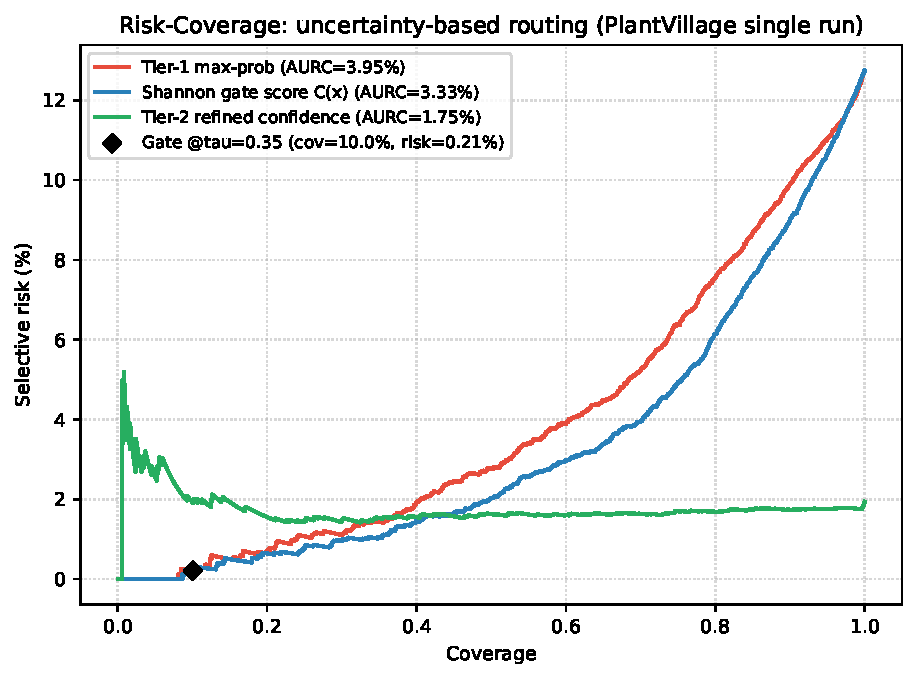
\includegraphics[width=0.96\linewidth]{fig_risk_coverage.pdf}
  \caption{Risk--coverage curves comparing raw Tier-1 maximum softmax probability, the dual-metric Shannon gate score $\mathcal{C}(\mathbf{x})$, and Tier-2 refined consensus confidence (canonical single run). The black diamond marks the deployed operating point at $\tau=0.35$ (10.0\% coverage at 0.21\% selective risk on this episode).}
  \label{fig:risk_coverage}
\end{minipage}\hfill
\begin{minipage}[b]{0.48\textwidth}
  \centering
  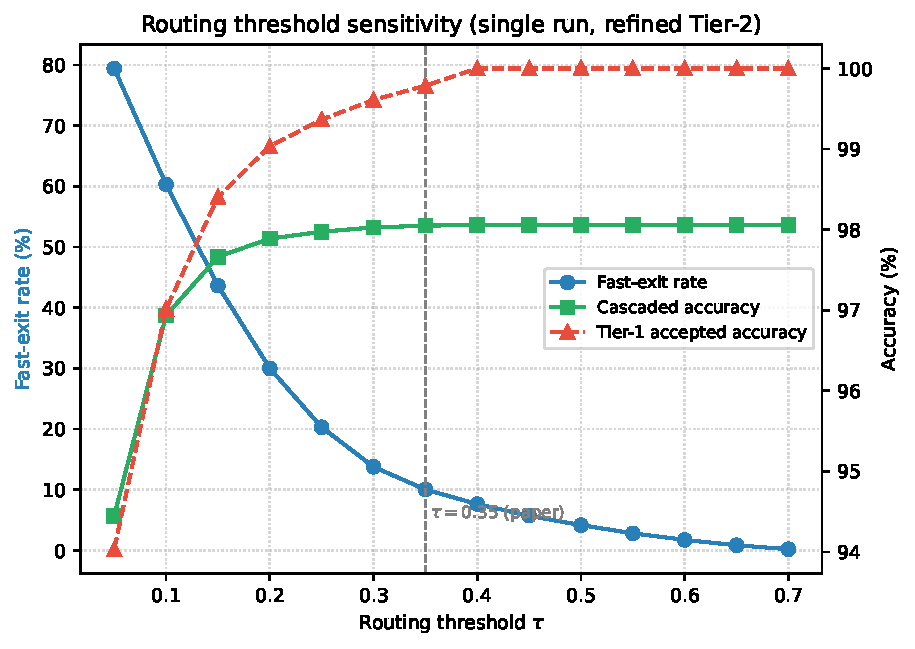
\includegraphics[width=0.96\linewidth]{fig_tau_sensitivity.pdf}
  \caption{Parametric routing-threshold sensitivity sweep across $\tau \in [0.05, 0.70]$ under refined Tier-2 inference. Blue circles (left axis) display fast-exit coverage (\%); green squares and red triangles (right axis) display full cascaded and Tier-1 accepted accuracies (\%). The vertical dashed line marks the deployed operating point ($\tau=0.35$).}
  \label{fig:tau_sensitivity}
\end{minipage}
\end{figure}

Table~\ref{tab:threshold_sweep} compares discrete routing policies across $\tau$. Aggressive policies ($\tau \le 0.20$) maximize fast-exit throughput (up to 61.76\% coverage and 99.83\,ms latency) but reduce Tier-1 accuracy below 99\%, allowing diseased leaves to escape undetected. Conservative policies ($\tau \ge 0.50$) ensure 100\% Tier-1 accuracy but restrict fast-exit coverage to only 5.15\%, diminishing latency benefits. Setting $\tau = 0.35$ balances these constraints, achieving 99.69\% Tier-1 accuracy with a 14.02\% fast-exit rate.

\begin{table}[htbp]
\caption{Selective routing policy sensitivity across gating threshold ($\tau$) sweeps.}
\label{tab:threshold_sweep}
\centering

\footnotesize
\setlength{\tabcolsep}{5pt}
\begin{tabularx}{\textwidth}{@{}>{\raggedright\arraybackslash}X *{4}{>{\centering\arraybackslash}p{2.3cm}}@{}}
\toprule
\textbf{Threshold Policy} & \textbf{Fast-Exit (\%)} & \textbf{Tier-1 Acc. (\%)} & \textbf{Cascaded Acc. (\%)} & \textbf{Latency (ms)} \\
\midrule
Aggressive ($\tau=0.10$) & 61.76$\pm$3.51 & 96.64$\pm$0.81 & 96.09$\pm$0.68 & 99.83$\pm$3.68 \\
Moderate ($\tau=0.20$) & 34.39$\pm$3.00 & 99.08$\pm$0.37 & 97.21$\pm$0.70 & 128.50$\pm$3.14 \\
\textbf{Deployed sweet spot ($\tau=0.35$)} & \textbf{14.02$\pm$2.25} & \textbf{99.69$\pm$0.41} & \textbf{97.36$\pm$0.69} & \textbf{149.84$\pm$2.36} \\
Conservative ($\tau=0.50$) & 5.15$\pm$1.42 & 100.00$\pm$0.00 & 97.28$\pm$0.86 & 159.13$\pm$1.48 \\
No fast path (monolithic Tier-2) & 0.00 & -- & 97.28$\pm$0.86 & 164.52 \\
\bottomrule
\end{tabularx}

\vspace{3pt}
\begin{minipage}{\textwidth}
\footnotesize
\textit{Notes.} Values are mean $\pm$ std over 30 Monte Carlo episodes. Bold marks the deployed operating point ($\tau=0.35$). Fast-exit coverage reflects the 30-episode mean over the 9,330-query stream.
\end{minipage}
\end{table}

Table~\ref{tab:tier_routing} reports the operational metrics across execution paths at this deployed operating point ($\tau=0.35$). The Tier-1 fast path (14.02\% coverage) executes in 59.78\,ms with 99.69\% accuracy and a false-negative rate (FNR) of 0.25\%. The Tier-2 escalated path (85.98\% coverage) executes in 164.52\,ms with 96.98\% accuracy. Compared to routing all queries through Tier-2 (164.52\,ms), cascaded execution reduces mean latency to 149.84\,ms (saving $\approx$15\,ms per diagnosis) while maintaining 97.36\% overall accuracy and a 0.79\% FNR.

\begin{table}[htbp]
\caption{Tier-separated performance, diagnostic escape rate, and latency breakdown at deployed gating threshold ($\tau=0.35$).}
\label{tab:tier_routing}
\centering

\footnotesize
\setlength{\tabcolsep}{5pt}
\begin{tabularx}{\textwidth}{@{}>{\raggedright\arraybackslash}X *{4}{>{\centering\arraybackslash}p{2.3cm}}@{}}
\toprule
\textbf{Execution Path} & \textbf{Coverage (\%)} & \textbf{Accuracy (\%)} & \textbf{FNR (\%)} & \textbf{Latency (ms)} \\
\midrule
Tier-1 fast path (accepted) & 14.02$\pm$2.25 & \textbf{99.69$\pm$0.41} & \textbf{0.25$\pm$0.52} & \textbf{59.78} \\
Tier-2 escalated path & 85.98$\pm$2.25 & 96.98$\pm$0.83 & 0.87$\pm$0.39 & 164.52 \\
\textbf{Cascaded deployment (full stream)} & \textbf{100.00} & \underline{97.36$\pm$0.69} & \underline{0.79$\pm$0.36} & \underline{149.84$\pm$2.36} \\
\bottomrule
\end{tabularx}

\vspace{3pt}
\begin{minipage}{\textwidth}
\footnotesize
\textit{Notes.} Values are mean $\pm$ std across 30 Monte Carlo episodes (single-view reference). Bold marks the best result per column; underline marks full-stream cascaded deployment.
\end{minipage}
\end{table}

\textbf{Streaming adaptation stability and hyperparameter sensitivity.} Table~\ref{tab:transductive_sensitivity} evaluates transductive recalibration across three design parameters over 30 episodes:
(i)~\emph{Support weighting} ($1\times$ to $10\times$): Accuracy remains stable across $[1\times, 5\times]$ ($97.42\%$ to $97.32\%$). Although $2\times$ achieves $97.44\%$, we deploy $3\times$ ($97.41\%$) because it yields the lowest variance ($\pm 0.71\%$) and provides a stronger inductive anchor against potential pseudo-label noise during continuous field deployment.
(ii)~\emph{Anchor confidence threshold}: Accuracy remains constant at $97.41\%$ across $[0.50, 0.70]$. We deploy $0.70$ to ensure pseudo-label purity against field clutter, as higher thresholds ($\ge 0.80$) induce anchor buffer starvation ($95.98\%$).
(iii)~\emph{Buffer capacity per class}: Accuracy reaches $97.41\%$ with $20$ anchors per class. While larger capacities ($40$ and $80$) offer slight accuracy increases ($+0.10$\,pp and $+0.26$\,pp), capping at $20$ captures over $99.7\%$ of maximum transductive gain while bounding buffer memory and preserving sub-second ($0.53$\,s) background matrix solving.
During continuous streaming with FIFO replacement, accuracy increases from $96\%$ to $97$--$98.6\%$ without error accumulation, confirming that FIFO eviction safely purges stale anchors.

\begin{table}[htbp]
\caption{Sensitivity of transductive accuracy to recalibration design constants (mean $\pm$ std over 30 identical episodes; single-view reference).}
\label{tab:transductive_sensitivity}
\centering

\footnotesize
\setlength{\tabcolsep}{4pt}
\begin{tabular*}{\columnwidth}{@{\extracolsep{\fill}}lcc}
\toprule
\textbf{Swept Configuration} & \textbf{Acc. (\%) ($\uparrow$)} & \textbf{Std ($\downarrow$)} \\
\midrule
\multicolumn{3}{@{}l}{\textit{Support weight} (threshold 0.70, 20 anchors/class)} \\
$1\times$ & 97.42 & 0.75 \\
$2\times$ & \textbf{97.44} & 0.73 \\
$3\times$ (deployed) & 97.41 & \textbf{0.71} \\
$5\times$ & 97.32 & 0.73 \\
$10\times$ & 97.21 & 0.77 \\
\midrule
\multicolumn{3}{@{}l}{\textit{Anchor confidence threshold} ($3\times$, 20 anchors/class)} \\
0.50 & \textbf{97.41} & \textbf{0.71} \\
0.60 & \textbf{97.41} & \textbf{0.71} \\
0.70 (deployed) & \textbf{97.41} & \textbf{0.71} \\
0.80 & 95.98 & 1.28 \\
0.90 & 95.39 & 1.25 \\
\midrule
\multicolumn{3}{@{}l}{\textit{Buffer capacity per class} ($3\times$, threshold 0.70)} \\
5 & 96.36 & 0.97 \\
10 & 96.97 & 0.85 \\
20 (deployed) & 97.41 & 0.71 \\
40 & 97.51 & \textbf{0.62} \\
80 & \textbf{97.67} & 0.83 \\
\bottomrule
\end{tabular*}

\vspace{3pt}
\begin{minipage}{\columnwidth}
\footnotesize
\textit{Notes.} Bold marks the best value in each parameter sweep; ties are shown in bold.
\end{minipage}
\end{table}

\textbf{Covariance conditioning and augmentation dynamics.} Table~\ref{tab:aug_sensitivity} analyzes how multi-view support generation affects Ledoit--Wolf shrinkage and covariance conditioning under scarce support ($K=5$). Pure replication collapses the shrinkage intensity ($\rho^* = 0.072$) and degrades covariance conditioning ($\kappa = 9.6\times10^3$) because identical copies introduce no new sample variance. In contrast, stochastic geometric augmentation (random flips and rotations) injects directional diversity into the feature space, reducing shrinkage intensity ($\rho^* = 0.258$) and the condition number ($\kappa = 1.4\times10^3$), which improves inductive accuracy from 95.08\% to 96.09\% and transductive accuracy from 97.37\% to 97.96\%. Photometric jitter contributes negligible directional variance ($\kappa = 5.5\times10^3$), confirming that geometric transforms drive numerical covariance stability. The 8-view transductive accuracy (97.96\%) exceeds the single-view reference (97.41\%), confirming that single-view reported results are conservative.

\begin{table}[htbp]
\caption{Sensitivity of covariance conditioning and accuracy to augmentation count and type (mean $\pm$ std over episodes; 8-view sweep implementation).}
\label{tab:aug_sensitivity}
\centering

\footnotesize
\setlength{\tabcolsep}{2pt}
\begin{tabular*}{\columnwidth}{@{\extracolsep{\fill}}lccccc}
\toprule
\textbf{Condition} & \textbf{$N$} & \textbf{$\rho^*$} & \textbf{$\kappa(\hat{\mathbf{\Sigma}})$ ($\downarrow$)} & \textbf{Ind.\ (\%) ($\uparrow$)} & \textbf{Trans.\ (\%) ($\uparrow$)} \\
\midrule
\multicolumn{6}{@{}l}{\textit{View count sweep ($v\in\{1,2,4,8\}$, 30 episodes)}} \\
$v=1$ & 55 & 0.573$\pm$0.005 & \textbf{5.7$\times10^{2}$} & 95.08$\pm$1.27 & 97.37$\pm$0.73 \\
$v=2$ & 110 & 0.580$\pm$0.009 & 5.9$\times10^{2}$ & 95.50$\pm$1.21 & 97.67$\pm$0.57 \\
$v=4$ & 220 & 0.420$\pm$0.012 & 8.8$\times10^{2}$ & 95.80$\pm$1.25 & 97.81$\pm$0.63 \\
$v=8$ (full expansion) & 440 & 0.258$\pm$0.008 & 1.4$\times10^{3}$ & \textbf{96.09$\pm$1.20} & \textbf{97.96$\pm$0.50} \\
\midrule
\multicolumn{6}{@{}l}{\textit{Augmentation type sweep ($v=8$, first 10 episodes)}} \\
Geometric only & 440 & 0.229$\pm$0.008 & 1.6$\times10^{3}$ & \textbf{95.99$\pm$1.26} & \textbf{97.92$\pm$0.40} \\
Photometric only & 440 & 0.104$\pm$0.002 & 5.5$\times10^{3}$ & 94.70$\pm$1.90 & 97.31$\pm$0.61 \\
Full pipeline & 440 & 0.257$\pm$0.009 & \textbf{1.4$\times10^{3}$} & 95.85$\pm$1.40 & 97.85$\pm$0.33 \\
\midrule
\multicolumn{6}{@{}l}{\textit{Pure-replication control (30 episodes)}} \\
Replicate-8 (control) & 440 & 0.072$\pm$0.001 & 9.6$\times10^{3}$ & 95.05$\pm$1.28 & 97.01$\pm$0.79 \\
\bottomrule
\end{tabular*}

\vspace{3pt}
\begin{minipage}{\columnwidth}
\footnotesize
\textit{Notes.} $N$ denotes total support representations ($N = C \times K \times v$). $\rho^*$ represents the analytical Ledoit--Wolf optimal shrinkage intensity parameter. $\kappa(\hat{\mathbf{\Sigma}})$ is the regularized covariance condition number ($\lambda_{\max}/\lambda_{\min}$); $(\downarrow)$ denotes lower is better (indicating superior numerical conditioning). Ind.\ and Trans.\ denote inductive and transductive accuracies; $(\uparrow)$ denotes higher is better. Bold marks the best result per column in each evaluation panel.
\end{minipage}
\end{table}

% -----------------------------------------------------------------------------
% 5.6 Physical Interpretability and Diagnostic Failure Analysis
% -----------------------------------------------------------------------------
\subsection{Physical Interpretability and Diagnostic Failure Analysis}
\label{sec:per_class}

Table~\ref{tab:per_class} and Fig.~\ref{fig:confusion} report the per-class performance metrics and row-normalized confusion matrix across all 9,330 test leaves on PlantVillage.

\begin{table*}[htbp]
\caption{BioDINO-Edge per-class diagnostic metrics across 11 novel foliar pathologies (9,330 test leaves, single-view reference).}
\label{tab:per_class}
\centering

\footnotesize
\setlength{\tabcolsep}{5pt}
\begin{tabularx}{\textwidth}{@{}>{\raggedright\arraybackslash}X *{4}{c}@{}}
\toprule
\textbf{Foliar Pathology Category} & \textbf{Precision ($\uparrow$)} & \textbf{Recall ($\uparrow$)} & \textbf{F1-Score ($\uparrow$)} & \textbf{Test Support} \\
\midrule
Apple Scab (\textit{Venturia inaequalis}) & 0.963 & 0.947 & 0.955 & 625 \\
Apple Black Rot (\textit{Botryosphaeria obtusa}) & 0.951 & 0.974 & 0.962 & 616 \\
Apple Cedar Rust (\textit{Gymnosporangium juniperi-virginianae}) & 0.975 & 0.993 & 0.983 & 270 \\
Apple Healthy Foliage & 0.988 & 0.981 & 0.985 & 1,640 \\
\midrule
Grape Black Rot (\textit{Guignardia bidwellii}) & 0.972 & 0.980 & 0.976 & 1,175 \\
Grape Esca (\textit{Phaeomoniella chlamydospora}) & 0.982 & 0.976 & 0.979 & 1,378 \\
Grape Leaf Blight (\textit{Pseudocercospora vitis}) & \textbf{1.000} & \underline{0.997} & \textbf{0.999} & 1,071 \\
Grape Healthy Foliage & 0.993 & \textbf{1.000} & \underline{0.996} & 418 \\
\midrule
Potato Early Blight (\textit{Alternaria solani}) & \underline{0.997} & 0.990 & 0.993 & 995 \\
Potato Late Blight (\textit{Phytophthora infestans}) & 0.990 & 0.972 & 0.981 & 995 \\
Potato Healthy Foliage & 0.839 & 0.993 & 0.910 & 147 \\
\midrule
\textbf{Macro Average / Total Support} & \textbf{0.968} & \textbf{0.982} & \textbf{0.974} & \textbf{9,330} \\
\textbf{Single-Run Accuracy} & \multicolumn{4}{c}{\textbf{98.06\%} (Peak Statistical Episode: \textbf{98.67\%})} \\
\bottomrule
\end{tabularx}
\end{table*}

\textbf{Per-class diagnostic performance and error distribution.} Across individual pathologies, BioDINO-Edge maintains high classification fidelity, achieving macro F1-scores above 0.95 for all evaluated diseases. For healthy foliage, recall remains high across species (0.981 to 1.000). Potato Healthy yields 0.993 recall and 0.839 precision under severe class imbalance (147 healthy vs.\ $\approx$2,000 infected leaves), ensuring that symptomatic foliage is reliably identified while minimizing missed infections.

\begin{figure}[htbp]
\centering
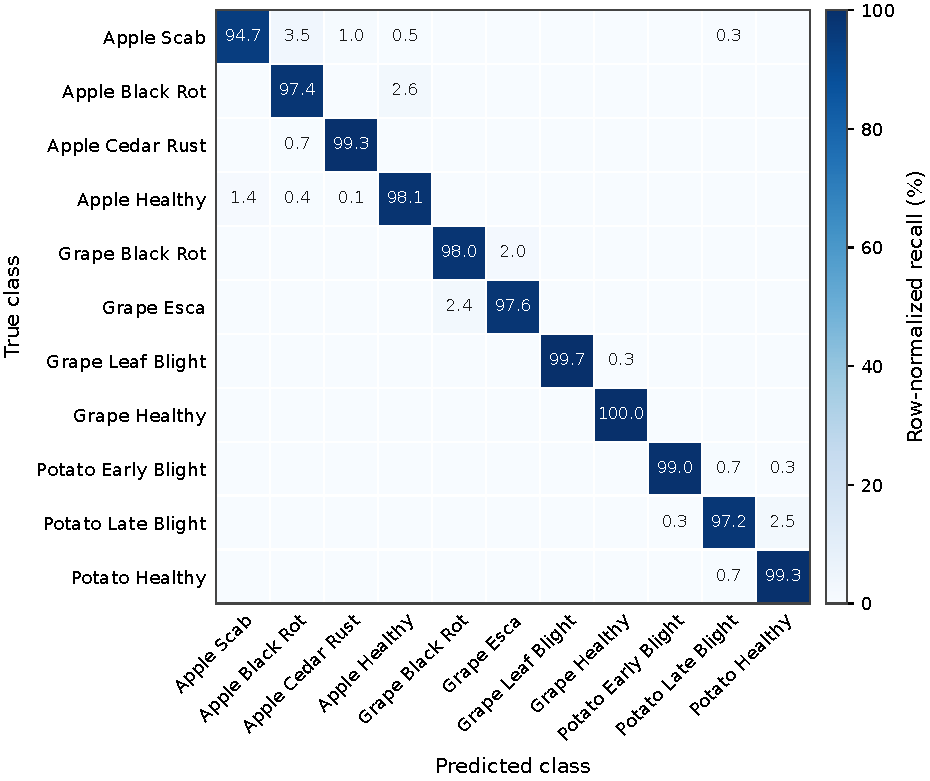
\includegraphics[width=0.82\columnwidth]{fig_confusion.pdf}
\caption{Row-normalized confusion matrix for BioDINO-Edge under transductive inference on the canonical PlantVillage split (9,330 test queries; 11 classes across Apple, Grape, and Potato). Rows represent ground-truth annotations; columns represent predictions. Diagonal entries indicate per-class recall (\%). Residual misclassifications concentrate strictly among pathologies of the same host species; cross-species confusion is negligible (0.021\%).}
\label{fig:confusion}
\end{figure}

\textbf{Diagnostic error patterns and epidemiological containment.} As visualized in Fig.~\ref{fig:confusion}, classification errors are strictly confined within the same botanical host species. Residual confusion occurs primarily between Apple Scab and Apple Black Rot (F1 0.955 and 0.962), where early necrotic spots share visual circularity and chlorotic borders, as well as between intermediate symptom stages of Grape Esca and Grape Black Rot (F1 0.979 and 0.976). Crucially for disease containment, cross-species confusion is near-zero: across 9,330 queries, only two apple scab leaves were misclassified as potato late blight (a 0.021\% error rate). Furthermore, the framework achieves a low false-negative rate of 0.702\% on this canonical split (0.79\% $\pm$ 0.36\% across 30 episodes), misclassifying only 50 out of 7,125 diseased leaves as healthy.
